%05/03 - Myriam
\part{Docking y dinámica molecular}
\chapter{Docking molecular}
Las áreas en las que se desarrolla el docking es el descubrimiento de fármacos y la química de productos naturales. Está el área de la quimioinformática, virtual screening y las técnicas QSAR que permiten predecir las propiedades físicas y químicas de moléculas. 

Hay cuatro bloques donde se aplica la modelización moléculas en el desarrollo de fármacos:
\begin{itemize}
\item Combinatorial Chemistry HTS: no se tiene conocimiento de la estructura de la proteína ni del ligando. Se crean bibliotecas y modelos 3D de la proteína.
\item Diseño de novo: se conoce la estructura de la proteína, pero no del ligando. Conocer la cavidad en la que se ensamble el ligando permite conocer los aminoácidos del bolsillo de interacción y diseñar así ligandos.
\item Diseño basado en la estructura del receptor: se concoe tanto la estructura de la proteína como de los ligandos. Se pretende conocer la interacción entre ambos.
\item Similitud de farmacóforo: se conoce la estructura de los ligandos, pero no de la proteína. El farmacóforo es el modelo que se compara con ligandos similares, enfrentándolo con bases de datos preexistentes.
\end{itemize}

Las técnicas experimentales principales para obtener la estructura de las proteínas son purificación de proteínas, cristalografía y resonancia magnética nuclear. Muchas proteínas están vinculadas a determinadas enfermedades. La idea es diseñar un fármaco que, al inhibir una proteína, se desencadena otra acción que puede ser beneficiosa para el tratamiento de la patología. 

\section{Screening and repositioning}
Lo principal es intentar crear una quimioteca de compuestos que se enfrenta a las proteínas de interés. Hay muchas formas de lograrlo, siendo una de ellas las predicciones ADMET. A día de hoy hay muchas herramientas ADMET para ver compuestos y si interesan o no para el estudio concreto. Poco a poco se crean bases de datos de interés para enfrentar a los receptores. El siguiente bloque es el docking molecular y la dinámica molecular, y por último los métodos de Poison-Bodman. El docking da una idea más global, pero este método hace una medición muy exacta de todas las interacciones de las proteínas con los ligandos. Esto se pasa a un programa de visualización y se sacan los compuestos que son idóneos para el tratamiento, pasando así a los experimentos in vitro.

\section{Docking molecular}
El docking es una técnica computaconal que permite conocer la interacción entre una proteína de interés y un ligando. Por ejemplo, en enfermedades neurodegenerativas, una proteína importante es Orai1. Se debe saber si hay un ligando que permita activar la función de la proteína y generar una respuesta biológica. Antes de gastar un dinero en un fármaco que pueda no funcionar, primero se mira computacionalmente si se puede producir actividad en cuanto a interacción. Se conocen las conformaciones del ligando en la cavidad proteica. Hay que conocer previamente el sitio de interacción de la proteína y dónde se quiere ensamblar el ligando. La herramienta quizás permite descubrir otros sitios de interacción que no se conocían. 

Hay dos tipos de interacción o acoplamiento:
\begin{itemize}
\item \textbf{Métodos basados en ligando:} se conoce la estructura del ligando, pero no se sabe a qué proteína se puede unir. Para ello, se enfrenta y se ve con qué proteína interacciona. Esto es importante en el high-throughput screening.
\item \textbf{Métodos basados en estructuras}: estos se usan principalmente para identificar las interacciones ligando-receptor, ya que se conoce la estructura de la proteína
\end{itemize}

El docking se basa en el modelo primario de acoplamiento de llave-cerradura. Se establecía que la proteína y el ligando eran entes rígidos e interesaba conocer la interacción. No obstante, las técnicas permitieron desarrollar el modelo de ajuste inducido, en el cual se veía que las estructuras eran más flexibles y dinámicas, cambiando de conformación para adaptarse al sustrato. 

\subsection{Docking rígido}
Aunque el modelo de Fisher sea un modelo anticuado, hay dockings donde se ponen la proteína y el ligando rígidos para ver si hay interacción entre ambos. El receptor rota y se traslada al ligando, pero no hay movimiento durante el cálculo. Permite simplificar ensayos para descartar rápidamente un compuesto.

\subsection{Docking semiflexible}
El ligando es flexible, pero la proteína no. La proteína se traslada y rota, pero se añaden los ángulos diedros. Uno de los softwares que permiten esto es Autodock. Este docking es bastante exhaustivo y permite concoer la conformación ideal del ligando. Es el que más se usa al poder usarse a nivel de usuario.

\subsection{Docking flexible}
Tanto la proteína como el ligando son flexibles. La precisión es muy buena, pero el tiempo de cálculo es muy amplio y es necesario ejecutarlo en un clúster. Al seleccionar la zona de interacción, estos residuos son los que se definen como flexibles, no es toda la proteína. 

\subsection{Información estructural del sitio activo}
Hay dos tipos de enfoque del docking molecular: acoplamiento a ciegas donde no se sabe si el ligando interacciona con la proteína. Programas como DiscoveryStudio calcula las cavidades que pueden ser de interés para poder hacer un estudio más centrado, ya que si se toma toda la proteína de golpe, los cálculos pueden saturarse por el gran tamaño. El acoplamiento específico se conoce el sitio y se centra en la cavidad el ligando. 

\section{Metodologías del docking}
Están los métodos sistemáticos y estocásticos. Autodock trabaja con los sistemáticos, pero con las nuevas versiones se está moviendo al estocástico. En el método sistemático, se explora la conformación del ligando, moviéndola hasta que encaja en la proteína. El movimiento se hace en todos los ángulos de rotación, siendo así menos específico. El método estocástico es al revés: las conformaciones se mueven de forma aleatoria para encontrar mínimos locales y globales. La metodología de estos softwares se suelen usar con espacios explorables grandes, mientras que los sistemáticos son más exhaustivos y es mejor utilizar con estructuras pequeñas. 

La formación de un complejo viene por la unión de proteína con ligando. Es un proceso termodinámico que tiende a un equilibrio, es decir, se consigue una energía de unión libre estable, muy baja. EL ligando ha conseguido estar a gusto en la cavidad proteica cuando se consigue esto. Para calcular las diferentes energías de unión se utilizan distintos algoritmos matemáticos.

\subsection{Algoritmo de búsqueda}
En el algoritmo de búsqueda exhaustiva, el programa busca todas las conformaciones posibles de ligando (que puede ser otra proteína) y proteína y busca los rotámeros ideales.

Algoritmo por fragmentación: corta el ligando en distintos fragmentos y los va insertando en la cavidad proteica. Cuando uno está a gusto, añade el siguiente. Así, se van añadiendo a cachos hasta encontrar la estructura ideal.

El algoritmo de Montecarlo (MC) es un método estocástico que cambia aleatoriamente los grados de liebrtad del sistema. La proteína y el ligando se van a unir, y el programa establece la energía de interacción. Si encuentra una interacción con una energía de afinidad mejor, el programa para. Si la siguiente no es muy buena, el programa vuelve a iniciar el cálculo. 

El algoritmo genético está basado en principios de evolución y selección natural para explorar el espacio. Los grados de libertad del ligando van a ser genes, y la conformación final son cromosomas. El programa "muta un gen", lo que equivale a cambiar la conformación. Si la mutación que se obtiene es positiva, el gen sobrevive, mientras que si es negativa, se deshecha. Todo esto es de forma metafórica; realmente no se evalúan genes.

A modo de resumen hasta ahora: tenemos la proteína y el ligando y se forma el complejo. Hay que elegir el programa más adecuado para lo que se quiere encontrar. Una vez que tenemos el cálculo hecho, hay que buscar la función de puntuación que calcula la energía de afinidad obtenida.

\section{Puntuación}
Docking genera millones de estructuras, por lo que es importante puntuarlas. El propio programa debe estimar las conformaciones correctas e incorrectas. Las funciones de puntuación no calculan la energía de afinidad, si no que es un dato estimado. Estas funciones están basadas en:
\begin{itemize}
\item \textbf{Campos de fuerza}: Calculan las interacciones entre los átomos del ligando y del receptor utilizando un conjunto de parámetros que describen las interacciones atómicas.
interacciones de Van der Waals y electrostáticas.
\item \textbf{Datos empíricos}: Se basan en datos experimentales (observaciones empíricas) y en parámetros ajustados estadísticamente para reflejar las interacciones entre el ligando y la proteína.
Se añaden enlace de hidrógeno, solvatación, hidrofobicidad y otros.
\item \textbf{Conocimiento}: Se apoyan en datos experimentales o literatura científica para desarrollar modelos de puntuación.
Asumen que los contactos estadísticamente más explorados se correlacionan con interacciones más favorables
\end{itemize}

Bases de datos para los fármacos son PubChem, ChEMBL, Drugbank y SINC. El programa de Schrödinger es muy completo, y hace un docking en el que se conoce el sitio de interacción (no puede ser ciego). También permite hacer dinámica molecular. Otro programa es MOE, el cual permite hacer estudios QSAR.

Bases de datos de proteínas principales son PDB y AlphaFold. Para modelar las proteínas se puede utilizar I-TASSER, Swiss-Model y AlphaFold. 

\begin{table}[h]
\centering
\begin{tabular}{l l}
Situación & Software reocmendado \\ \hline
Proteína con homólogos en PDB & Swiss-Model o I-Tasser \\
Proteína sin estructura previa & AlphaFold \\
Predicciones rápidas y sencillas & Swiss-Model \\
Predicciones detalladas y refinadas & I-TASSER \\
Acceso a GPUs y predicciones muy precisas & AlphaFold
\end{tabular}
\end{table}

\section{Esquema general de trabajo}
Se trabaja con ficheros pdb del receptor y ligando. Se convierten en ficheros pdbqt que contiene coordenadas, cargas parciales y tipos de átomos. Esto se puede ajustar al tamaño y posición del grid, es decir, la parte de la proteína que nos interesa para el docking.

\section{Práctica}
El ligando es el fichero jnj.pdb, y la proteína es P2X7-SWISSMODEL.pdb. Con esto localizado, vamos al programa Avogadro. Al descargar un ligando o fármaco, no es real, es plano. Por ello, Avogadro permite minimizar la estructura a una más real. 

Al final hemos utilizado la tolcapona. En PubChem hemos buscado tolcapone y descargado la estructura 3D en SDF. Esto lo abrimos en Avogadro. En la barra superior hay un botón con una E y una flecha hacia abajo (tres botones a la izquierda de Tool Settings). Seleccionamos el campo de fuerza MMFF94 con 4 pasos por update y pulsamos start. 

\begin{figure}[h]
\centering
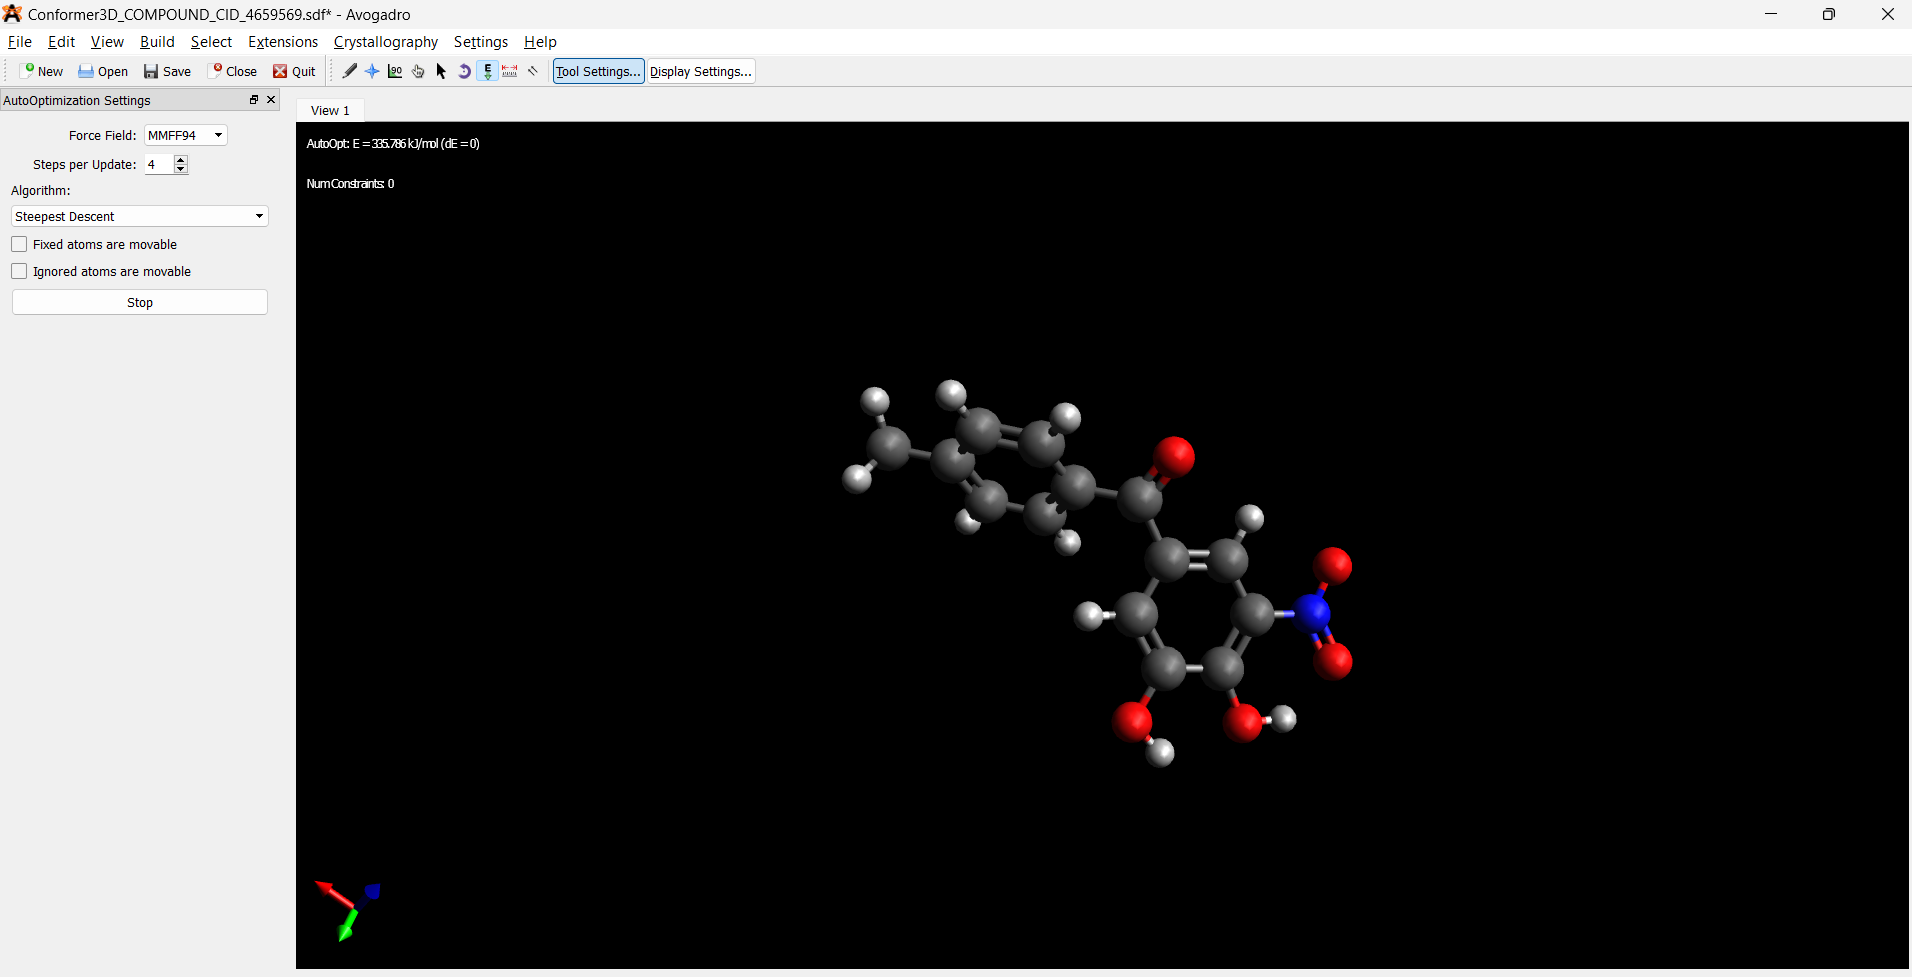
\includegraphics[width = 0.7\textwidth]{figs/avogadro-tolcapona.png}
\end{figure}

Una vez terminado, lo guardamos en formato PDB y abrimos Chimera. Ahí abrimos P2X7-Swissmodel.pdb. A continuación vamos a Tools > Surface/Binding Analysis > Dock Prep. Es importante que esté marcada la opción de "Add hydrogens" y "Add charges". Este programa trabaja con estructuras en formato Mol2 para docking, por lo que esa opción también debe estar habilitada. En la siguiente pantalla debe considerar todos los enlaces de hidrógeno. Como la histidina es el aminoácido más complejo de protonar in silico, se especifica (lo dejamos por defecto, pero en estudios in silico es importante revisarlo). En cuanto a las cargas, utilizamos los residuos estándar AMBER ff14SB. La siguiente pestaña es para guardar el archivo. Le ponemos un nombre (que en este caso es p2x7\_dockprep) y lo guardamos.

En una nueva sesión abrimos jnj y volvemos a ir a Dock Prep. Repetimos lo mismo, pero en el campo de fuerzas cambiamos AM1-BCC por Gasteiger. Vemos que la carga neta es +1 y volvemos a asegurarnos de que el método sea Gasteiger. Guardamos el ligando en formato mol2. 

Cerramos la sesión y abrimos los dos ficheros .mol2 que acabamos de generar. Debemos alejarnos, ya que las dos estructuras no están juntas. Habiendo leído bibliografía previa, sabemos que el ligando se une a la proteína en la zona de beta láminas y no en las hélices alfa. Nos interesa que el ligando se una en el centro del poro o en alguna zona lateral. Ahora vamos a Favorite > Model Panel y se desmarca la proteína para poder mover el ligando. Ahora lo podemos colocar cerca del poro. Una vez terminado, Tools > Surface/Binding Analysis > Autodock Vina > Browse y ponemos un nombre de fichero. Después de aceptar seleccionamos como receptor la proteína y ligando nuestro ligando. En Receptor search volume options ponemos un 10 en todas las filas para que aparezca la caja en cualquier sitio. Al pulsar la ruedecita del centro del ratón, se selecciona toda la proteína directamente. También podemos mover la caja independientemente y ajustarla manualmente. Idealmente, la parte de las hélices alfa está fuera. Si siempre trabajamos con la misma proteína, conviene apuntarnos las coordenadas buenas que se han actualizado en el panel anterior. En opciones de receptor deben estar todos en verdadero salvo "ignore all non-standard residues", que debe estar en falso. El resto lo dejamos por defecto salvo Number of Binding Models, que lo subimos a 10. En executable location, debemos asegurarnos de que esté el path del ejecutable (que suele estar en C:/Program Files(x86)/The Scripp Research Institute/Vina/vina.exe).

\begin{figure}[h]
\centering
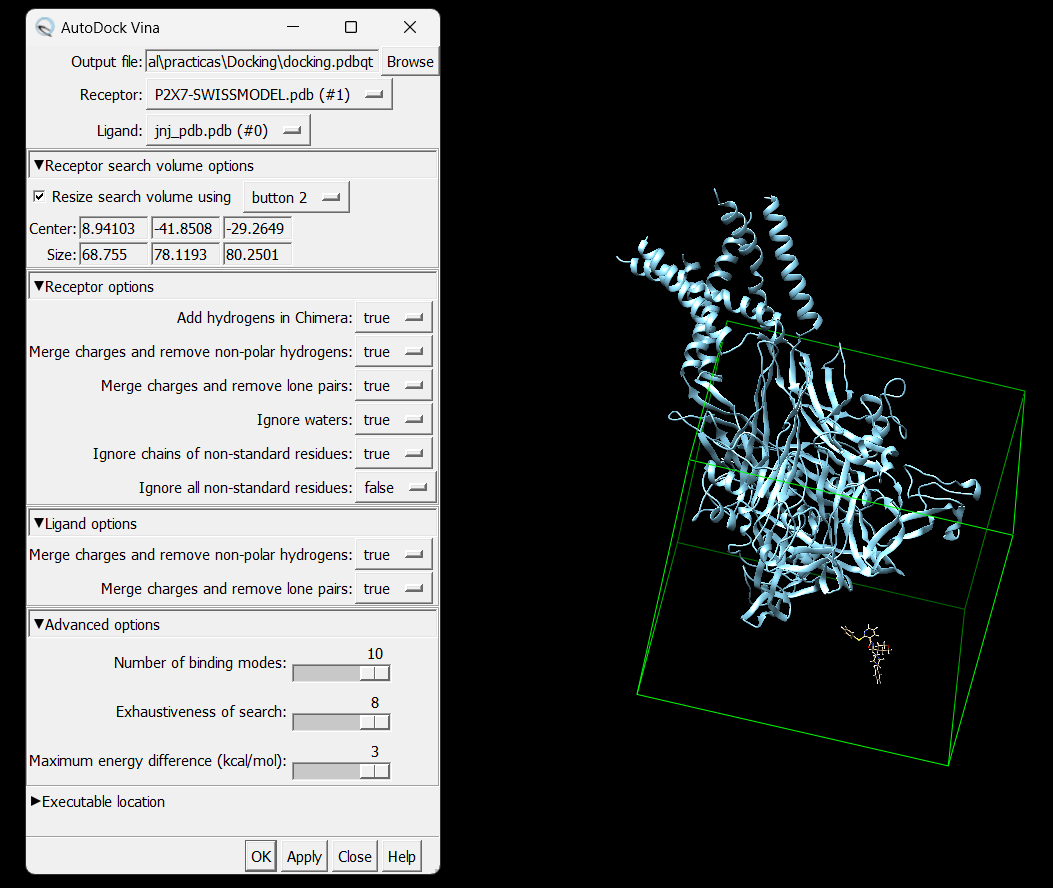
\includegraphics[width = 0.7\textwidth]{figs/docking.png}
\end{figure}

Una vez terminado, aparece una tabla con las distintas uniones ordenadas. Las interacciones deberían estar a no más de 5 $\AA$ y se debe revisar manualmente que el docking es real y no esté en mitad de la proteína. Se puede mirar en PyMOL abriendo los ficheros docking.pdbqt y docking.receptor.pdbqt. 